\chapter{Шагающий робот}
{\bfseries Анонс:}\\\\
Знакомство с плоскими шарнирными механизмами. Построение шагающего робота на основе стопоходящей машины Чебышева.\\\\
{\bfseries Цели:}
\begin{itemize}
	\item{}{\bfseries Обучающие:} Ознакомить с понятием шарнирных механизмов. Обучить построению шагающего робота. 
	\item{}{\bfseries Развивающая:} Развитие познавательного интереса учащихся.\\
\end{itemize}	
{\bfseries Ход занятия:}\\\\
\begin{tabular}[h!]{lll}
	{\hyperlink{lesson22x1}{1. Организационный момент}}&{Презентация}&{(15 мин)}\\
	{\hyperlink{lesson22x2}{2. Шарнирные механизмы}}&{Игра}&{(20 мин)}\\
	{\hyperlink{lesson22x3}{3. Робот-стопоход}}&{Практика}&{(50 мин)}\\
	{\hyperlink{lesson22x4}{4. Соревнования  шагающих роботов*}}&{Игра}&{(30 мин)}\\
\end{tabular}\\\\

{\hypertarget{lesson22x1}{\blackBlueText{I. Организационный момент}}}\\\\	

В заключение конструкционной части предлагается поговорить немного о шарнирных механизмах и построить шагающего робота. 

Построение шагающего робота само по себе уже является сложной задачей и может быть дано в качестве практикума на весь остаток занятия, после разговора о шарнирных механизмах. В случае сильных групп занятие можно дополнить соревнованиями шагающих роботов.\\\\
\clearpage
{\hypertarget{lesson22x2}{\blackBlueText{II. Шарнирные механизмы}}}\\\\

Как нарисовать прямую линию? Вопрос кажется очень странным , но для инженеров викторианской эпохи инженеров это была крайне важная  проблема. Она возникла из необходимости ограничить движение поршня в паровой машине, заставить его двигаться строго по прямой линии.  Например,  в паровом двигателе Ньюкомена (рис.) для этого использовалась цепи. Но с помощью цепи можно только тянуть поршень, но не толкать, поэтому при дальнейшей разработке двигателей этот подход оказался неприменим.\\\\

\greenText{Подробнее, спросить Диму}\\\\

\begin{figure}[h!]
	\begin{center}
		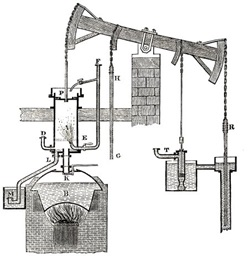
\includegraphics[width=0.92\linewidth]{chapters/chapter22/images/1}
		\caption{}
		\label{ris:image22x1}
	\end{center}
\end{figure}

Итак, под «рисованием прямой линии» инженерами прошлых веков понималось создание плоского механизма для ограничения  движения механических соединений для перемещения по прямой линии.

Первое «прямило» было изобретено Джеймсом Уаттом, вошедшим в историю изобретением паровой машины. Работая над машиной, он столкнулся с такой проблемой - как связать поршень с маховым колесом, чтобы вращение колеса сообщало поршню прямолинейное движение. В своих письмах, он так описывал идею своего механизма:

«The convexities of the arches, lying in contrary directions, there is a certain point within the connecting-lever, [the movement of] which has very little sensible variation from a straight line».

Отметим, что Уатт не утверждал, что его прямило создает идеально прямую линию.

\begin{figure}[h!]
	\begin{center}
		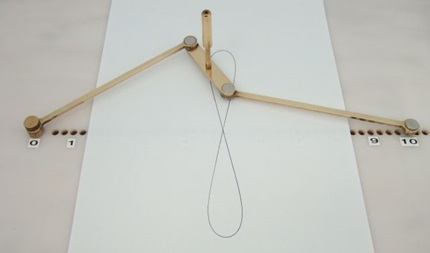
\includegraphics[width=1\linewidth]{chapters/chapter22/images/2}
		\caption{Прямило Уатта.}
		\label{ris:image22x2}
	\end{center}
\end{figure}

После открытия Уатта был разработан целый ряд механизмов, которые приблизительно вычерчивающих прямую. Одним из известнейших ученых, работавший в этой области, русский математик Пафнутий Львович Чебышев (1821--1894). и его много проектов это самый известный. Интересно, что Пафнутий Львович сам вытачивал на станках свои шарнирные механизмы, в основном из бронзы. В Санкт-Петербурге, в музее истории науки до сих пор хранится шкаф с его моделями. На протяжении многих лет он занимался как усовершенствованиями прямила, так и другими шарнирными механизмами, но был твердо убежден, что механическая система никогда не сможет вопроизвести точную прямую линию.
\clearpage
\begin{figure}[h!]
	\begin{center}
		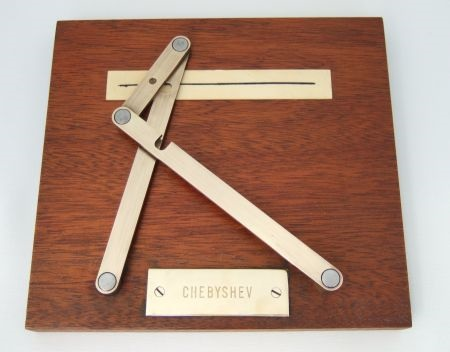
\includegraphics[width=1\linewidth]{chapters/chapter22/images/3}
		\caption{}
		\label{ris:image22x3}
	\end{center}
\end{figure}

Однако, его ученик Липман Липкин опроверг это утверждение, сумев построить в 1868 году прямило Липкина, создающее идеально прямую линию. В части иностранной литературы пальму первенстве в построении точного прямила отдают офицеру инженерного корпуса французской армии Поселье (Charles Nicolas Peaucellier). Он действительно, первым описал идею подобного механизма в письме в 1864 году, однако не указал никаких технических подробностей. В 1870 г он опубликовал подробню статью, уже со ссылкой на Липкина.
\clearpage
\begin{figure}[h!]
	\begin{center}
		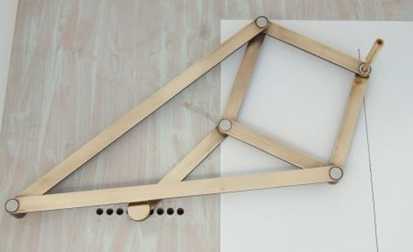
\includegraphics[width=1\linewidth]{chapters/chapter22/images/4}
		\caption{}
		\label{ris:image22x4}
	\end{center}
\end{figure}

{\slshape Математические выкладки, показывающие, что прямило Липкина действительно дает абсолютно точную прямую линию, очень красивы и показывают связь абстрактных понятий с реальными механизмами. В 10--11 классах можно посветить отдельное занятие математике и созданию прямила Липкина. Рекомендуемую литературу для подготовки подобного занятия можно найти в Приложении.}

Позднее был изобретен еще ряд прямил, дающих точную прямую линию:

\begin{figure}[h!]
	\begin{center}
		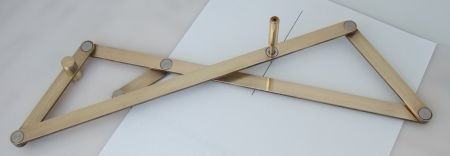
\includegraphics[width=1\linewidth]{chapters/chapter22/images/5}
		\caption{}
		\label{ris:image22x5}
	\end{center}
\end{figure}	
\clearpage
\begin{figure}[h!]
	\begin{center}
		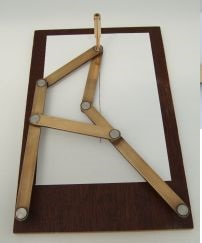
\includegraphics[width=1\linewidth]{chapters/chapter22/images/6}
		\caption{}
		\label{ris:image22x6}
	\end{center}
\end{figure}	
\clearpage
\begin{figure}[h!]
	\begin{center}
		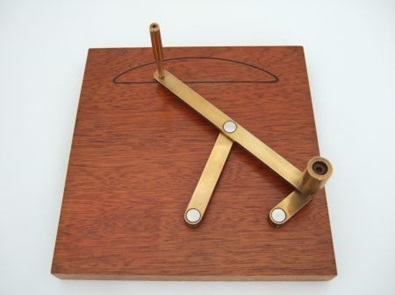
\includegraphics[width=0.99\linewidth]{chapters/chapter22/images/9}
		\caption{}
		\label{ris:image22x9}
	\end{center}
\end{figure}

Интересно, что в XXI веке математиками была доказана теорема о подписи~--- существует плоский шарнирный механизм, подделывающий Вашу подпись сколь угодно точно.\\\\

{\hypertarget{lesson22x3}{\blackBlueText{III. Робот-стопоход}}}\\\\

{\slshape Задача достаточно сложна для учащихся даже после нижеследующих объяснений механизма работы, но неизменно вызывает восторг при окончательной реализации, а так же позволяет закрепить основные принципы построения прочных конструкций.}

В основу конструкции робота положен стопоходящий механизм П.Л.Чебышева (рис.~\ref{ris:image22x7}), так же родившийся из задачи «прямой линии». С его помощью можно преобразовать движение по окружности в движение по траектории, напоминающей шляпку гриба (рис.~\ref{ris:image22x8}). При этом прямая часть траектории соответствует половине окружности. Таким образом, если закрепить на одном моторе два стопоходящих механизма в противоположных положениях, то всегда хотя бы одна нога будет стоять на земле (рис.~\ref{ris:image22x10}). 

В конструкции  робота используются два блока из двух ног, закрепленных на одном моторе.


\begin{figure}[h!]
	\begin{minipage}[h!]{0.5\linewidth}
		\begin{center}
			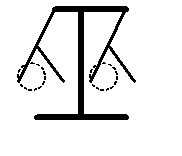
\includegraphics[width=1\linewidth]{chapters/chapter22/images/7}
			\caption{Механизм Чебышева.}
			\label{ris:image22x7}
		\end{center}
	\end{minipage}
	\begin{minipage}[h!]{0.5\linewidth}
		\begin{center}
			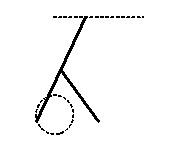
\includegraphics[width=1\linewidth]{chapters/chapter22/images/8}
			\caption{Преобразование траектории.}
			\label{ris:image22x8}
		\end{center}
	\end{minipage}
\end{figure}

\begin{figure}[h!]
	\begin{center}
		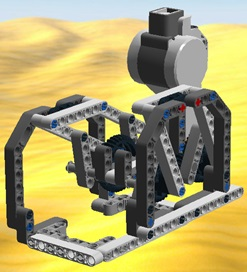
\includegraphics[width=0.67\linewidth]{chapters/chapter22/images/10}
		\caption{Две ноги на моторе.}
		\label{ris:image22x10}
	\end{center}
\end{figure}

\noindent\underline{Задание:} Построить робота на основе механизма Чебышева. Разрешается использовать любую справочную литературу, так же учащимся выдан файл с LDD моделью «ног» робота (как на рис.~\ref{ris:image22x10}).
\clearpage
{\hypertarget{lesson22x4}{\blackBlueText{IV. Соревнования шагающих роботов*}}}\\\\

В качестве усложнения задачи можно предложить шагающему  роботу выполнить все те же самые действия, что и трехколесной тележке ранее. А именно могут быть проведены:

\begin{enumerate}
	\item Гонки по линии шагающих роботов. 
	\item Сумо шагающих роботов.
	\item Подъем шагающих роботов по лестнице.
	\item Перешагивание роботами препятствий.
	\item Гонки многоногих шагающих роботов.
\end{enumerate}

Пример робота для ориентирования в лабиринте и сбивания банок:

\begin{figure}[h!]
	\begin{center}
		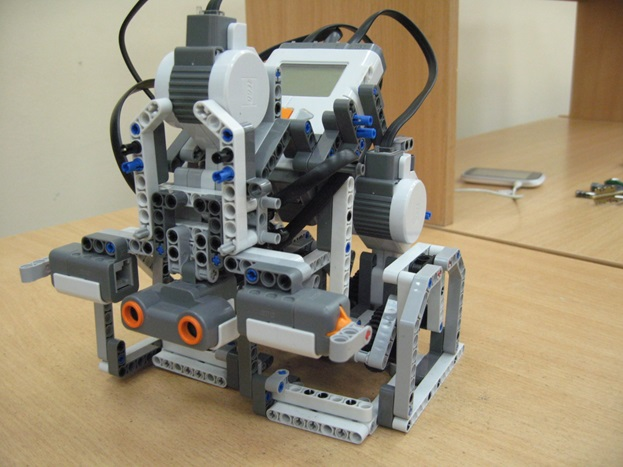
\includegraphics[width=0.86\linewidth]{chapters/chapter22/images/11}
		\caption{Две ноги на моторе.}
		\label{ris:image22x11}
	\end{center}
\end{figure}

\noindent В приложение:\\\\
\href{http://web.mat.bham.ac.uk/C.J.Sangwin/howroundcom/straightline/index.html}{\whiteBlueText{\underline{http://web.mat.bham.ac.uk/C.J.Sangwin/howroundcom/straightline/index.html}}}\\\\
\href{http://ebooks.library.cornell.edu/cgi/t/text/text-idx?c=math;cc=math;rgn=main;view=text;idno=kemp009}{\whiteBlueText{\underline{http://ebooks.library.cornell.edu/cgi/t/text/text-idx?c=math;cc=math;rgn=main;view=text;idno=kemp009}}}\\\\
\href{http://klu.narod.ru/diss1-053-3.html}{\whiteBlueText{\underline{http://klu.narod.ru/diss1-053-3.html}}}